\chapter{Additional material on Matched Filter}

\section{Low-pass FIR filter design}
\label{sec:matched_filter_fir}

To optimise the frequency response of a digital filter, we can use the Parks-McClellan algorithm, where one finds a set of $N$ real coefficients that give the best response for the specified pass-band and order of the filter \cite{McClellan2005}.

Taking the detector ticks as the time unit, the Nyquist frequency will simply be $1/2 \ \mathrm{ticks^{-1}}$. The current implementation of the filter seems to have as pass-band the range $[0,0.1] \ \mathrm{ticks^{-1}}$. This can be seen in Fig. \ref{fig:filter_comp}, where I show the power spectrum, in decibels, of that filter implementation (blue solid line). The Park-McClellan algorithm finds the optimal Chebyshev FIR filter \cite{Weinberg1960} taking as input the boundaries of the target pass-band and stop-band, which can be written in the form:
\begin{equation}
	\left\{ \begin{array}{c}
		\left[0, f_{c}\right] \\
		\left[ f_{c} + \delta f, f_{N}\right]
	\end{array} \right. ,
\end{equation}
where $f_{c}$ is the cut-off frequency, $\delta f$ is the transition width and $f_{N}$ is the aforementioned Nyquist frequency. A filter with a similar behaviour to the previous one can be obtained by setting $f_{c} = 0$ and $\delta f = 0.1 \ \mathrm{ticks}^{-1}$. The response of the resulting filter is also shown in Fig. \ref{fig:filter_comp} (blue solid line). Notice that the suppression of the stop-band is enhanced for this optimal filter. For comparison, I include the power response of the filter obtained by taking the integer part of the coefficients resulting from the Parks-McClellan method (red dashed line). One can see that it does not suppress that much the stop-band, in a similar way to the current implementation of the filter.

\begin{figure}[h!]
	\centering
	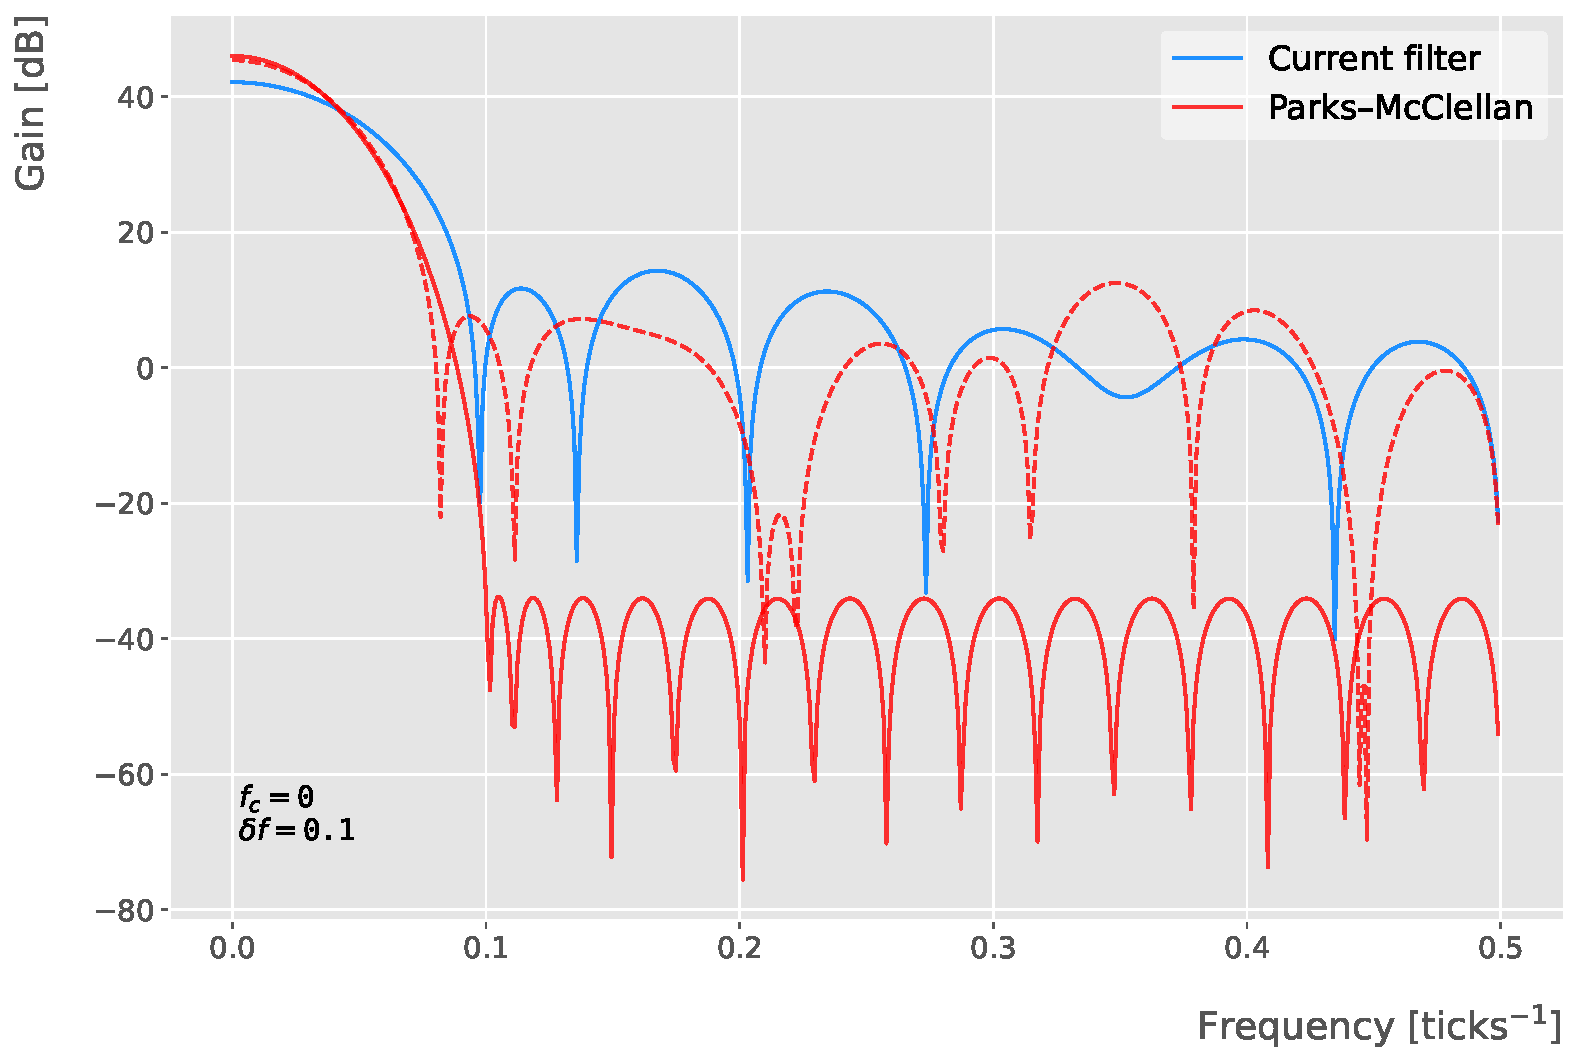
\includegraphics[width=0.8\linewidth]{Images/Matched_Filter/filter_comp}
	\caption[Power spectra for the current low-pass FIR filter and the optimal filter obtained using the Parks-McClellan algorithm.]{Power spectrum in decibels for the current implementation of the low-pass FIR filter in \texttt{dtp-firmware} (blue line), compared to the response of an optimal filter obtained using the Parks-McClellan algorithm for the same pass-band (red line). Also for comparison I include the spectrum of the optimal filter when taking only the integer part of the coefficients (red dashed line).}
	\label{fig:filter_comp}
\end{figure}

At this point, I tried to improve the performance of the FIR filter using the Park-McClellan method, i.e. maximise the overall S/N, using the available data captures. I did so by varying the values of the two quantities that parametrise the pass-band and stop-band, the cut-off frequency $f_{c}$ and the transition width $\delta f$.

\begin{figure}[t]
	\centering
	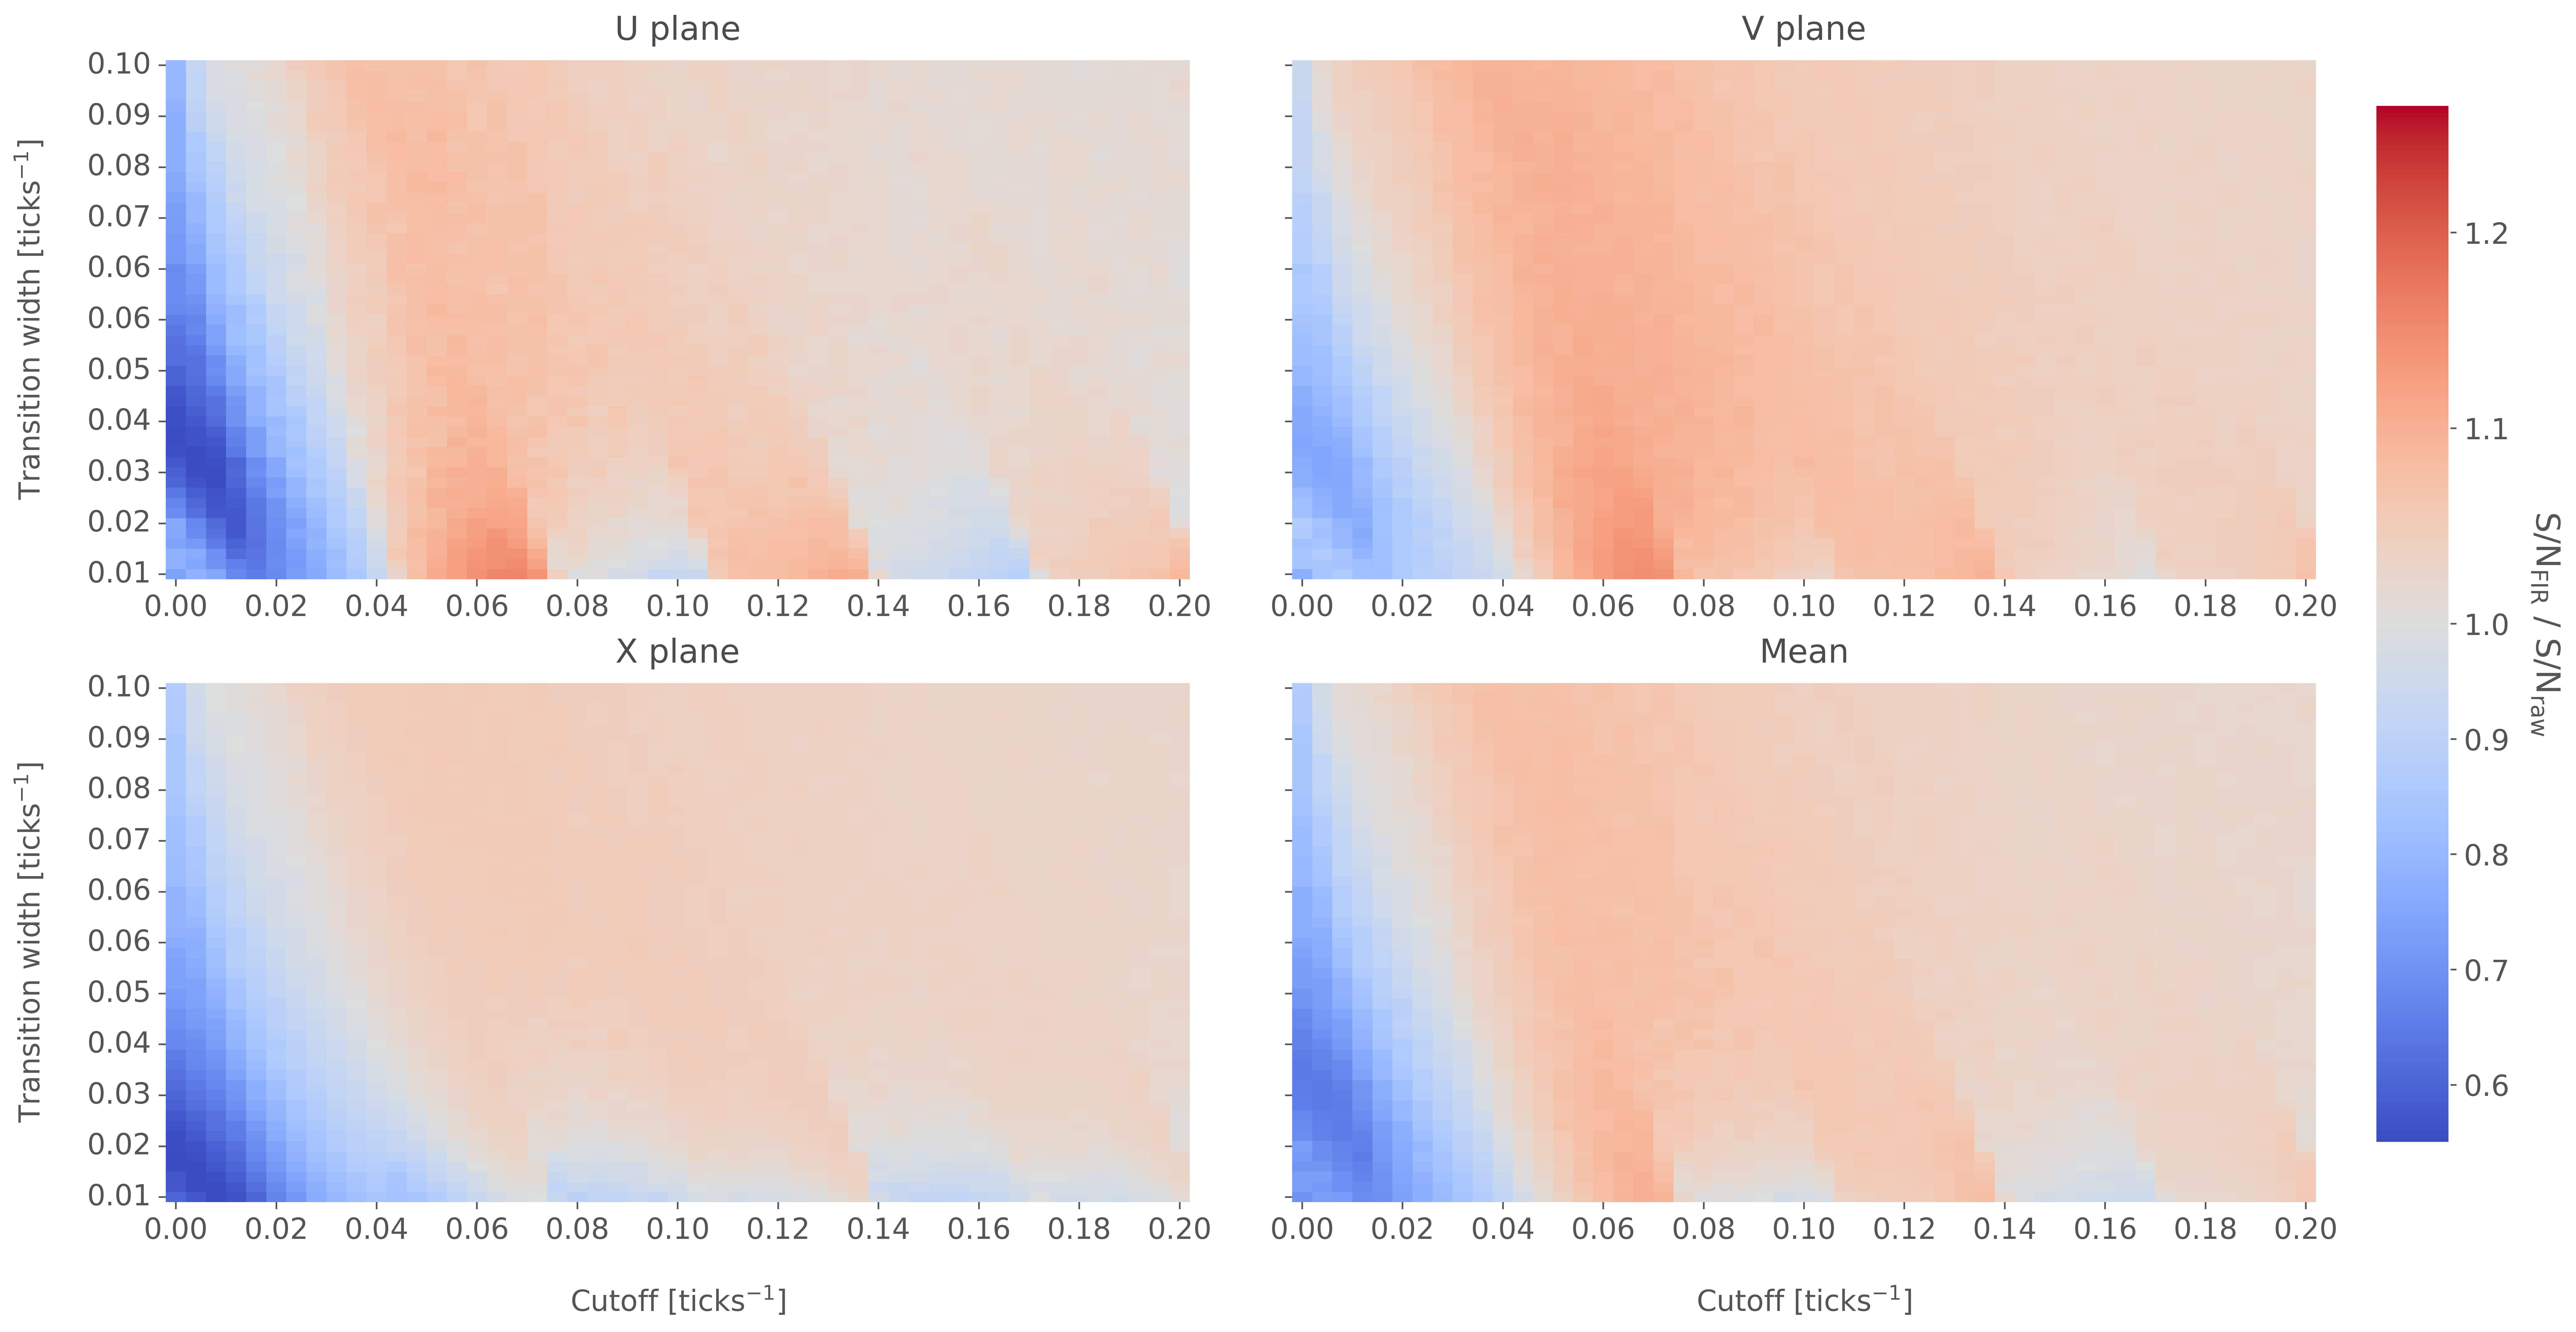
\includegraphics[width=1\linewidth]{Images/Matched_Filter/pm_fir_opt.png}
	\caption[Relative change in the S/N of the ProtoDUNE-SP raw data capture for different values of the cutoff frequency $f_{c}$ and the transition width $\delta f$.]{Relative change in the S/N for the ProtoDUNE-SP raw data capture \texttt{felix-2020-07-17-21:31:44}, using different values of the cutoff frequency $f_{c}$ and the transition width $\delta f$. The optimal Chebyshev filters were applied using just the integer part of the coefficients given by the Parks-McClellan algorithm.}
	\label{fig:fir_opt}
\end{figure}

\begin{figure}[t]
	\centering
	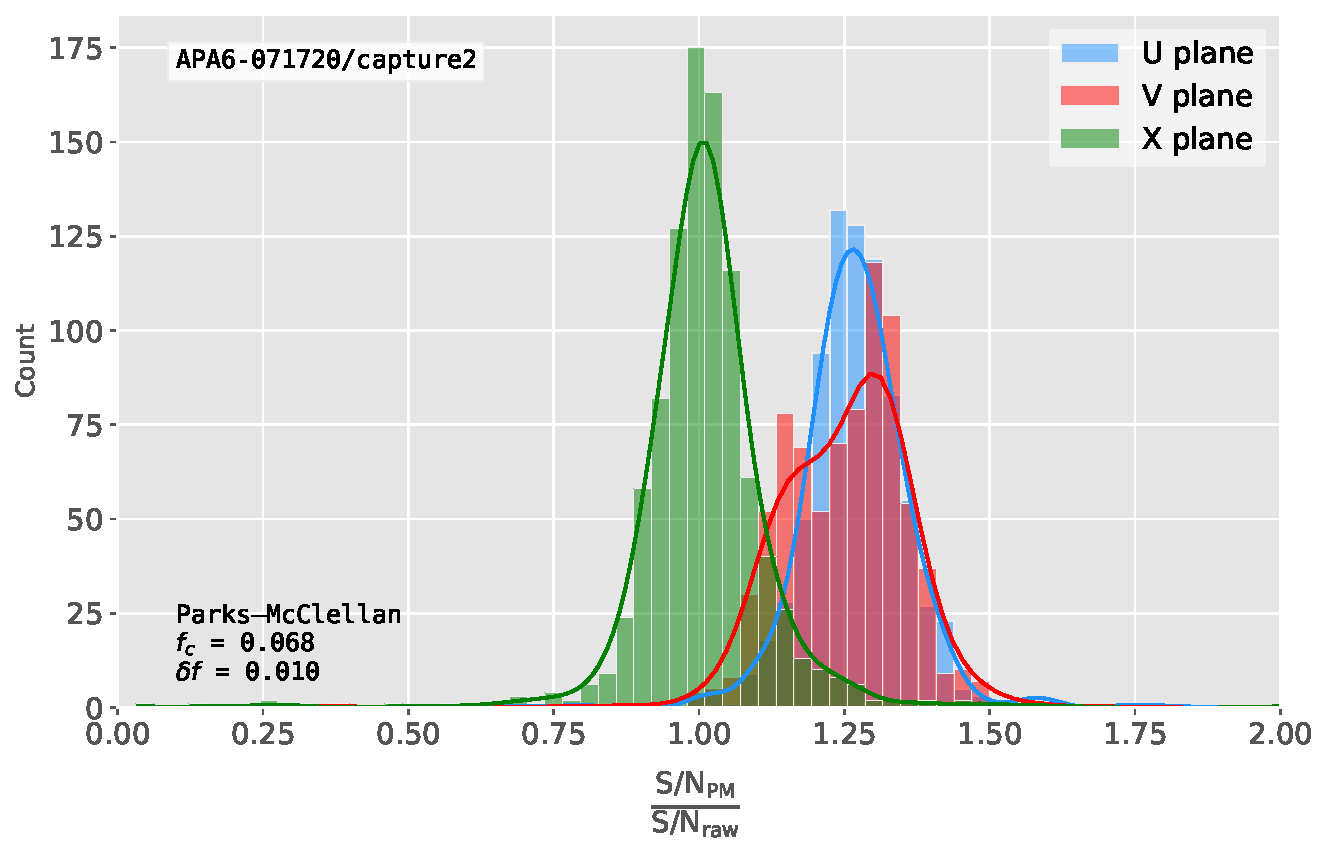
\includegraphics[width=0.85\linewidth]{Images/Matched_Filter/pm_fir_perf}
	\caption[Distribution of the relative change of the S/N on the different wire planes after the optimal FIR filter was applied.]{Distribution of the relative change of the S/N on the different wire planes from the ProtoDUNE-SP raw data capture \texttt{felix-2020-07-17-21:31:44} after the optimal Chebyshev filter was applied. The filter was computed with the Parks-McClellan algorithm using a cutoff of $f_{c} = 0.068 \ \mathrm{ticks}^{-1}$ and a transition width $\delta f = 0.010 \ \mathrm{ticks}^{-1}$.}
	\label{fig:fir_best}
\end{figure}

Figure \ref{fig:fir_opt} shows the average relative change in the S/N (i.e. the ratio between the value of the S/N after and before the filtering) for capture \texttt{felix-2020-07-17-21:31:44}, when using filters designed with the Parks-McClellan algorithm for the specified values of the cut-off frequency $f_{c}$ and the transition width $\delta f$, restricted to integer values for the filter coefficients. One can clearly distinguish different regions where we get an improvement of up to a factor of $1.35$ for the U plane. For large values of $f_{c} + \delta f$ the ratio tends to $1$, as expected. In that limit the width of the stop-band goes to $0$, meaning that no frequencies are filtered out and thus the waveform remains the same.

As it can be seen in Fig. \ref{fig:fir_opt} (bottom right panel) the configuration which gives the best mean performance for the three planes is $f_{c} = 0.068 \ \mathrm{ticks}^{-1}$ and $\delta f = 0.010 \ \mathrm{ticks}^{-1}$. We can use these to see how the filter affects the different channels. Figure \ref{fig:fir_best} shows the distribution of the S/N improvement values for all the channels in the raw ADC capture \texttt{felix-2020-07-17-21:31:44}, separated by wire plane, after the optimal Chebyshev filter was applied. One can see that there is a clear improvement for both U and V induction planes, obtaining a mean change of $1.25$ and $1.30$ for them, respectively. However, in the case of the X collection plane the distribution peaks around $1$, meaning that an important fraction of channels in that plane get a slightly worse S/N after the filter is applied. This is not a big issue, as the S/N for collection channels is usually much higher than the one for induction channels.

The results I obtained optimising the low pass filter with the Parks-McClellan method are promising. Nonetheless, the improvement found is rather marginal. Thus, I explored alternative approaches to the filtering problem, which may yield better outputs. This way, I found a possible solution in matched filters. By construction, this kind of filters offer the best improvement on the S/N.

\section{Matched filter impulse-response function}
\label{sec:matched_filter_impulse}

Given a known signal sequence $s(t)$ and another (a priori unknown) noise sequence $n(t)$, the input signal can be written as:
\begin{equation}\label{2.4.1}
	x(t) = s(t) + n(t).
\end{equation}

Now, considering a linear time-invariant filter, whose impulse-response function I will refer to as $h(t)$, one can write the output signal as:
\begin{equation}\label{2.4.2}
	\begin{split}
		y(t) &= x(t)*h(t)\\
		&= \left(s(t) + n(t)\right)*h(t)\\
		&= y_{s}(t) + y_{n}(t),
	\end{split}
\end{equation}
where $y_{s}(t)$ and $y_{n}(t)$ are simply the outputs of the filter due to the signal and the noise components respectively.

The goal of the matched filter is to detect the presence of the signal $s(t)$ in the input sample $x(t)$ at a certain time $t_{0}$, which effectively means that we need to maximise the S/N at that given time. This way, what one wants is to have a filter which gives a much bigger output when the known signal is present than when it is not. Putting it in other words, the instantaneous power of the signal output $y_{s}(t)$ should be much larger than the average power of the noise output $y_{n}(t)$ at some time $t_{0}$.

For the case of the filtered signal, one can easily re-write it as an inverse Fourier transform:
\begin{equation}\label{2.4.3}
	y_{s}(t) = \frac{1}{2\pi} \int_{-\infty}^{\infty} \mathrm{d}\omega \ H(\omega) S(\omega) \mathrm{e}^{i \omega t},
\end{equation}
where $H(\omega)$ and $S(\omega)$ are the Fourier transforms of the impulse-response function (i.e. the transfer function of the filter) and of the input signal, respectively.

Now, focusing on the noise part, we can use the Wiener-Khinchin theorem \cite{Goodman1985} to write the mean power of the noise after filtering as:
\begin{equation}\label{2.4.4}
	E|y_{n}(t)|^{2} = \frac{1}{2\pi} \int_{-\infty}^{\infty} \mathrm{d}\omega \ |H(\omega)|^{2} S_{n}(\omega),
\end{equation}
where $S_{n}(\omega)$ is the power spectral density of the noise.

Having these, one can write the instantaneous S/N at time $t_{0}$ as:
\begin{equation}\label{2.4.5}
	\begin{split}
		\left(\frac{S}{N}\right)_{t_{0}} &= \frac{|y_{s}|^{2}}{E|y_{n}(t)|^{2}}\\
		&= \frac{1}{2\pi} \frac{\left|\int_{-\infty}^{\infty} \mathrm{d}\omega \ H(\omega) S(\omega) \mathrm{e}^{i \omega t_{0}}\right|^{2}}{\int_{-\infty}^{\infty} \mathrm{d}\omega \left|H(\omega)\right|^{2} S_{n}(\omega)}.
	\end{split}
\end{equation}

Once we have this expression, we need to find its upper limit to determine what would be the optimal choice for the transfer function. For this, we use the Cauchy-Schwarz inequality, which in the present case takes the form:
\begin{equation}\label{2.4.6}
	\left|\int_{-\infty}^{\infty} \mathrm{d}x \ f(x) g(x)\right|^{2} \leq \int_{-\infty}^{\infty} \mathrm{d}x \ \left|f(x)\right|^{2} + \int_{-\infty}^{\infty} \mathrm{d}x \ \left|g(x)\right|^{2},
\end{equation}
for any two analytical functions $f(x)$ and $g(x)$. One can prove that making the choice:
\begin{equation}\label{2.4.7}
	\begin{split}
		&f(x) = H(\omega) \sqrt{S_{n}(\omega)}\mathrm{e}^{i \omega t_{0}},\\
		&g(x) = \frac{S(\omega)}{\sqrt{S_{n}(\omega)}},
	\end{split}
\end{equation}
leads to the following upper bound for the S/N:
\begin{equation}\label{2.4.8}
	\left(\frac{S}{N}\right)_{t_{0}} \leq \frac{1}{2\pi}\int_{-\infty}^{\infty} \mathrm{d}\omega \  \frac{\left|S(\omega)\right|^{2}}{S_{n}(\omega)}.
\end{equation}

From Eqs. (\ref{2.4.5}), (\ref{2.4.6}) and (\ref{2.4.7}) one can also derive the form of the transfer function such that the upper bound is exactly reached \cite{Dwork1950}:
\begin{equation}\label{2.4.9}
	H(\omega) \propto \frac{S^{*}(\omega) \mathrm{e}^{-i \omega t_{0}}}{S_{n}(\omega)}.
\end{equation}

From this last expression we can clearly see the way the matched filter acts. As the transfer function is proportional to the Fourier transform of the signal it will try to only pick the frequencies present in the signal \cite{Wainstein1962}.

The matched filter transfer function can be greatly simplified if the input noise is Gaussian. In that case, the power spectral density of the noise is a constant, so it can be re-absorbed in the overall normalisation of the transfer function. Moreover, considering that the input signal is a real function, one can simply set $S^{*}(\omega) = S(-\omega)$, which gives:
\begin{equation}\label{2.4.10}
	H(\omega) \propto S(-\omega) \mathrm{e}^{-i \omega t_{0}}.
\end{equation}

For a discrete signal, one can think of the input and impulse-response sequences as vectors. Then, the matched filter tries to maximise the inner product of the signal and the filter while minimising the output due to the noise by choosing a filter vector orthogonal to the latter. In the case of additive noise, that leads to the impulse-response vector:
\begin{equation}\label{2.4.11}
	h = \frac{1}{\sqrt{s^{\dagger} R_{n}^{-1} s}} \ R_{n}^{-1} s,
\end{equation}
where $s$ is a reversed signal template sequence of length $N$ equal to the order of the filter and $R_{n}$ is the covariance matrix associated with the noise sequence $n$. For the Gaussian noise case, the covariance matrix is simply the unit matrix, so the above expression simplifies again to:
\begin{equation}\label{2.4.12}
	h = \frac{s}{|s|}.
\end{equation}

\begin{figure}[t]
	\begin{subfigure}{0.5\textwidth}
		\centering
		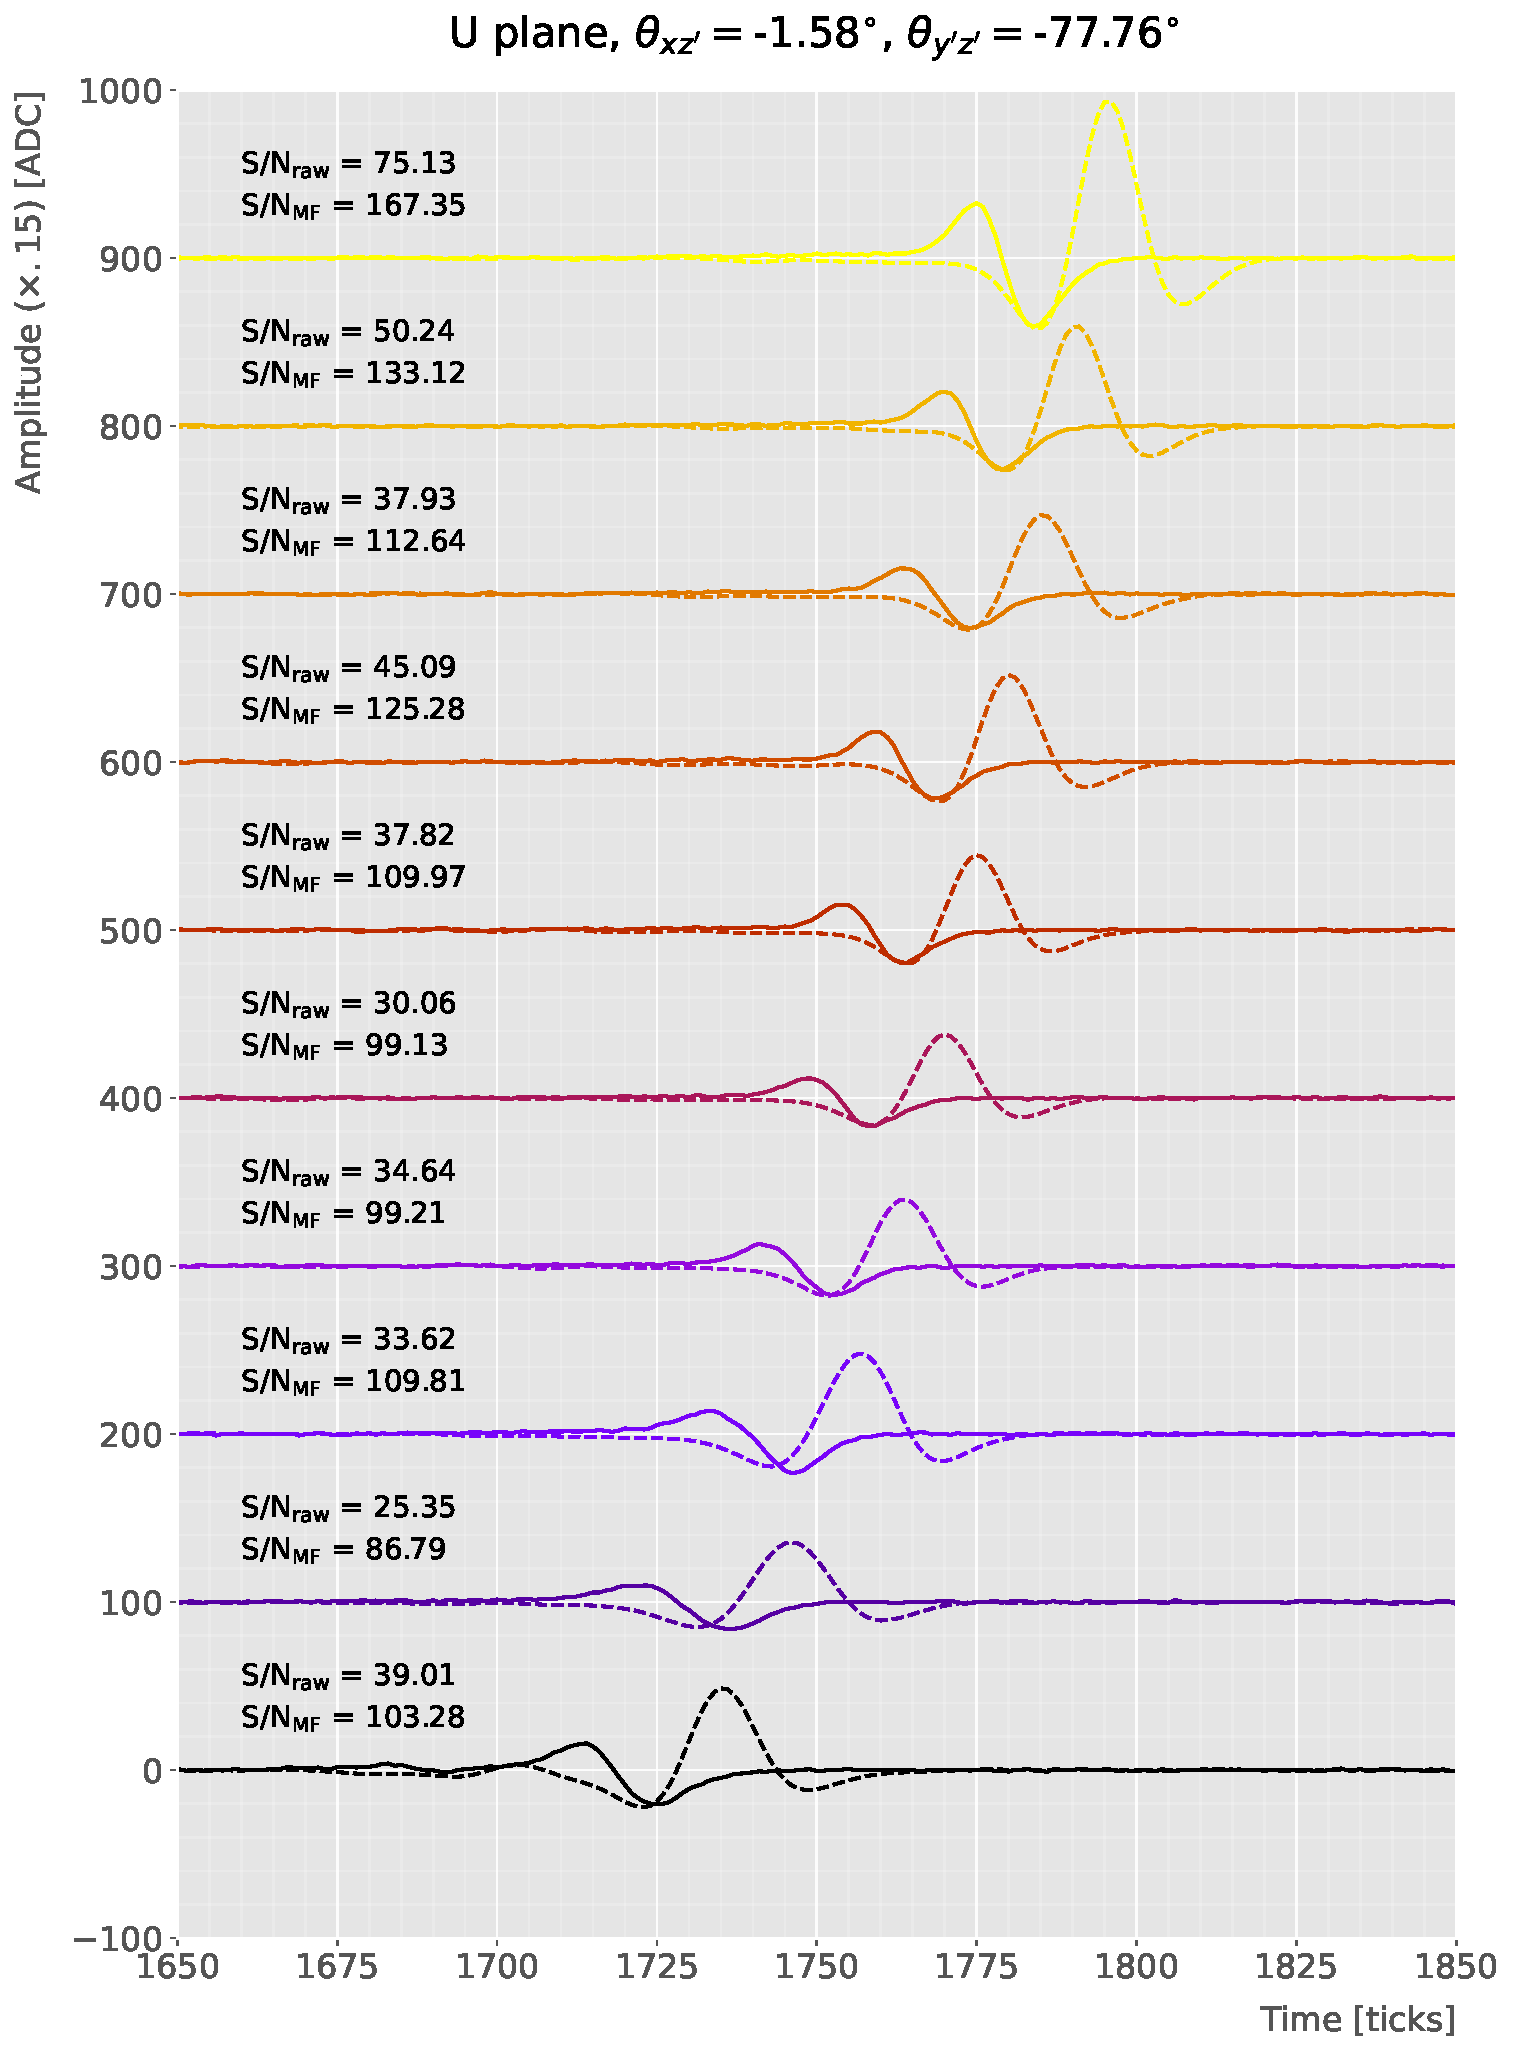
\includegraphics[width=.99\linewidth]{Images/Matched_Filter/evt_xz_0_yz_90_U}
	\end{subfigure}
	\begin{subfigure}{0.5\textwidth}
		\centering
		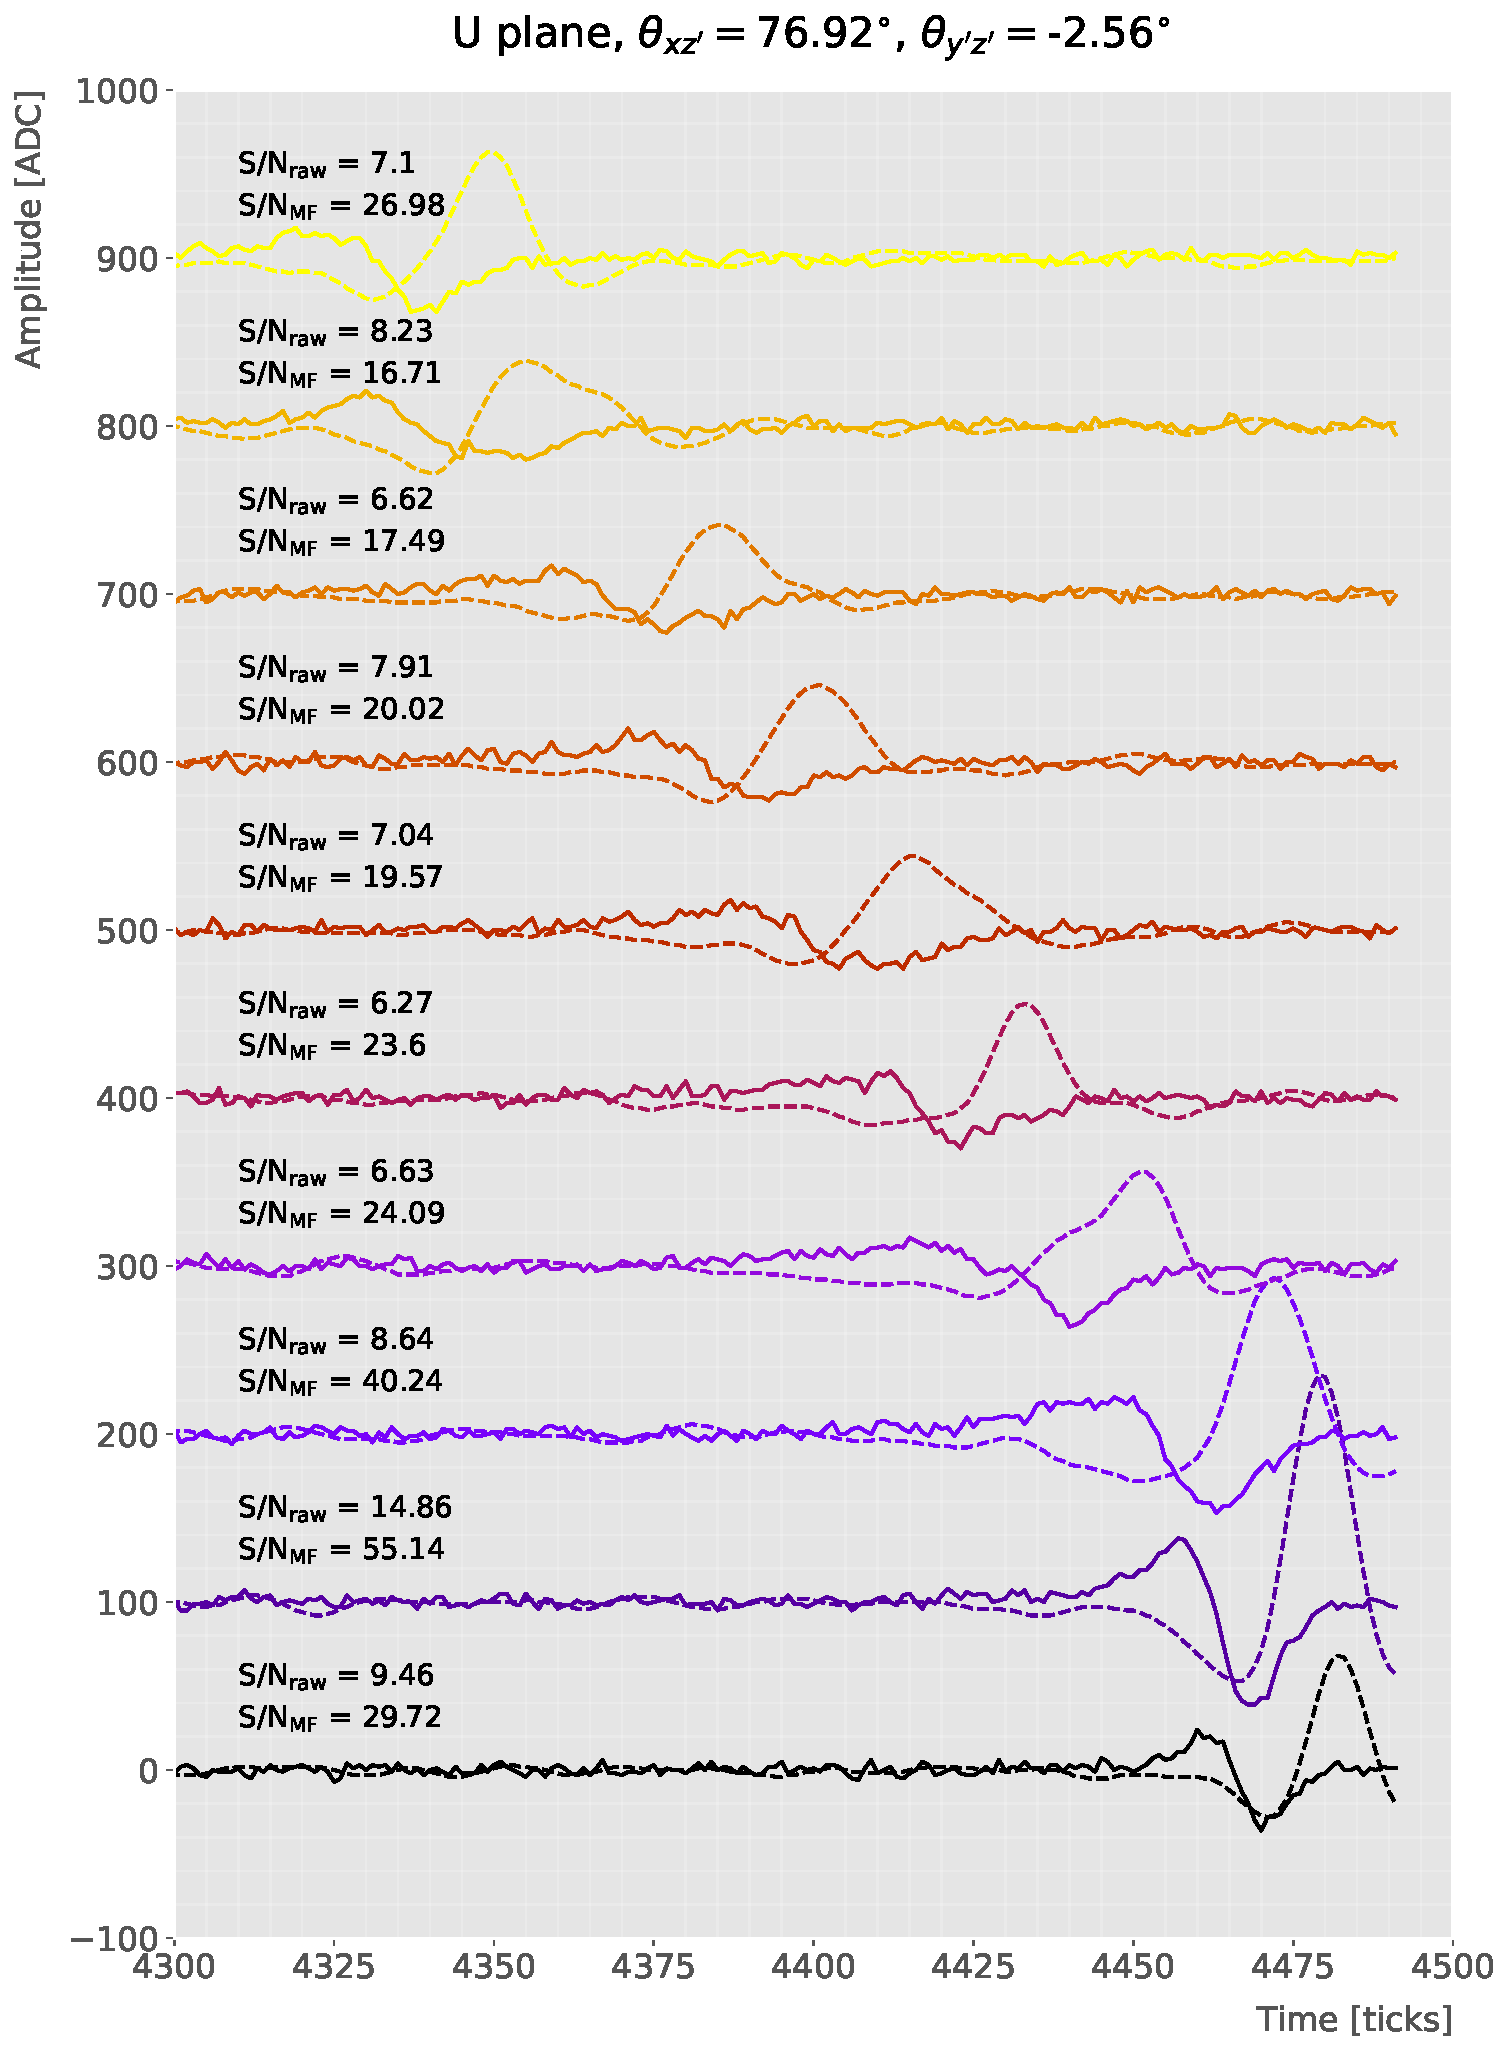
\includegraphics[width=.99\linewidth]{Images/Matched_Filter/evt_xz_90_yz_0_U}
	\end{subfigure}
	\caption[Waveforms for two muon events, one parallel to the APA and to the wires in the U plane and other normal to the APA plane and perpendicular to the U plane wires.]{Selected consecutive waveforms corresponding to two monoenergetic $E_{k} = 100 \ \mathrm{MeV}$ muon events, one is parallel to the APA and to the wires in the U plane (left panel) and the other is normal to the APA plane and perpendicular to the U plane wires (right panel). The solid lines represent the raw waveforms whereas the dashed lines correspond to the waveforms after the matched filter was applied. The waveforms on the left panel have been scaled by a factor of $0.15$ to have similar amplitudes to the ones on the right panel.}
	\label{fig:example_orientation}
\end{figure}

\section{Distortion and peak asymmetry}
\label{sec:A.5}

As a case study using the MC sample, I select two of the simulated $E_{k} = 100 \ \mathrm{MeV}$ monoenergetic muon events. With respect to the U induction plane, one is parallel to the APA (low $\theta_{xz'}$) and to the wires (high $\theta_{y'z'}$) and the other is normal to the APA plane (high $\theta_{xz'}$) and perpendicular to the wires (low $\theta_{y'z'}$). As expected from the results on the angular dependence discussed above, the former has a higher S/N (both before and after the filtering) when compared to the latter. An interesting thing to notice about these two samples is that, even though one has a much larger S/N than the other, it is the one with the smallest S/N the one that gets a more significant averaged S/N improvement. In Tab. \ref{tab:case} I include all the relevant parameters of these two $E_{k} = 100 \ \mathrm{MeV}$ muon events, namely the angles with respect to the $xy'z'$ reference frame, the values of the S/N, the S/N change and also the so-called peak asymmetry $\Delta_{peak}$, that I will define next.

\begin{figure}[t]
	\begin{subfigure}{0.5\textwidth}
		\centering
		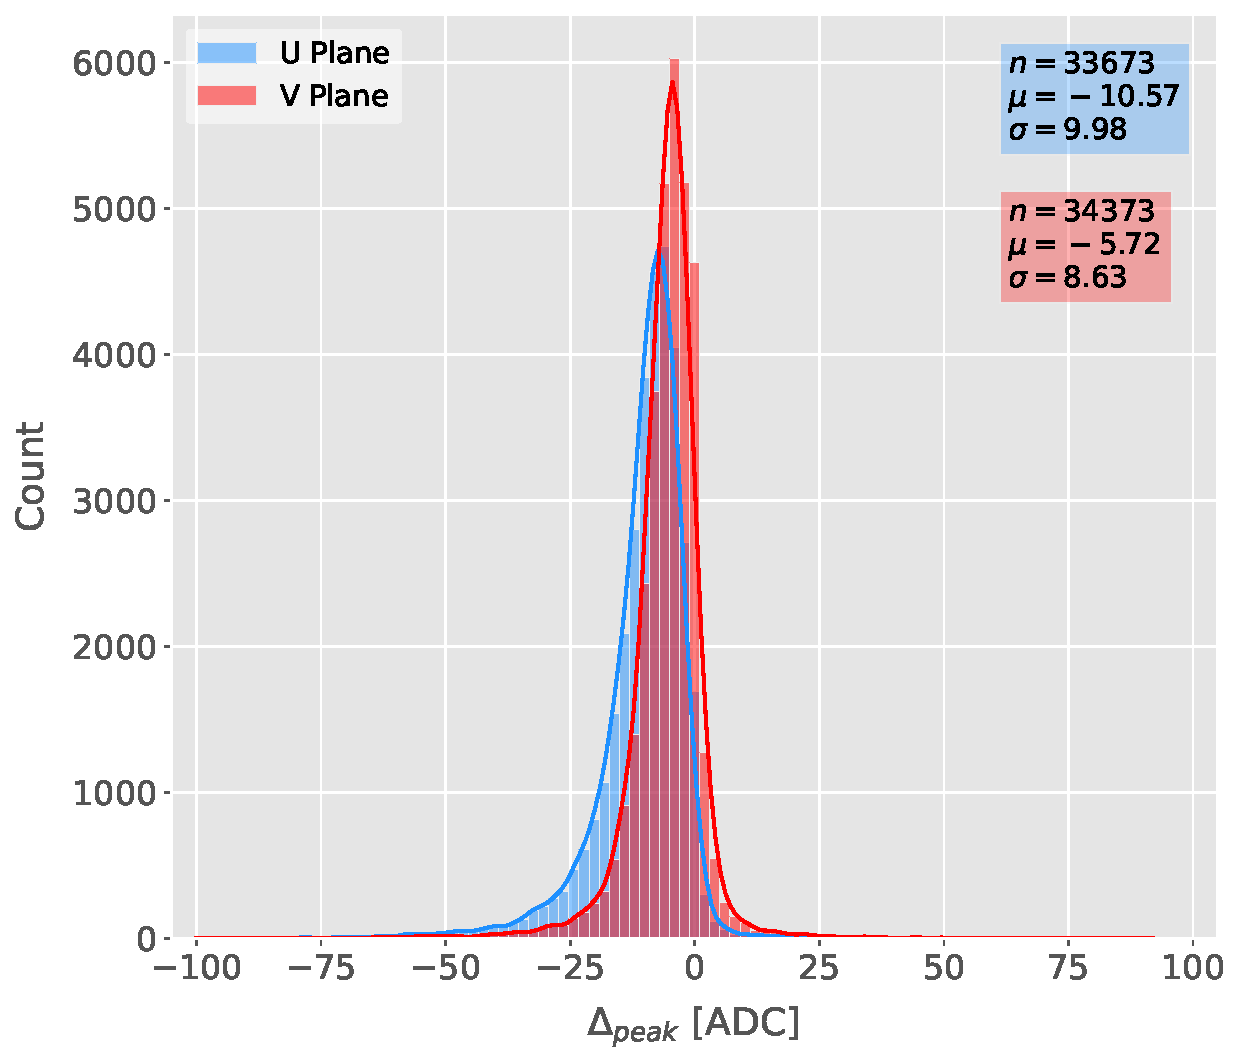
\includegraphics[width=.99\linewidth]{Images/Matched_Filter/deltaPeak_dist}
	\end{subfigure}
	\begin{subfigure}{0.5\textwidth}
		\centering
		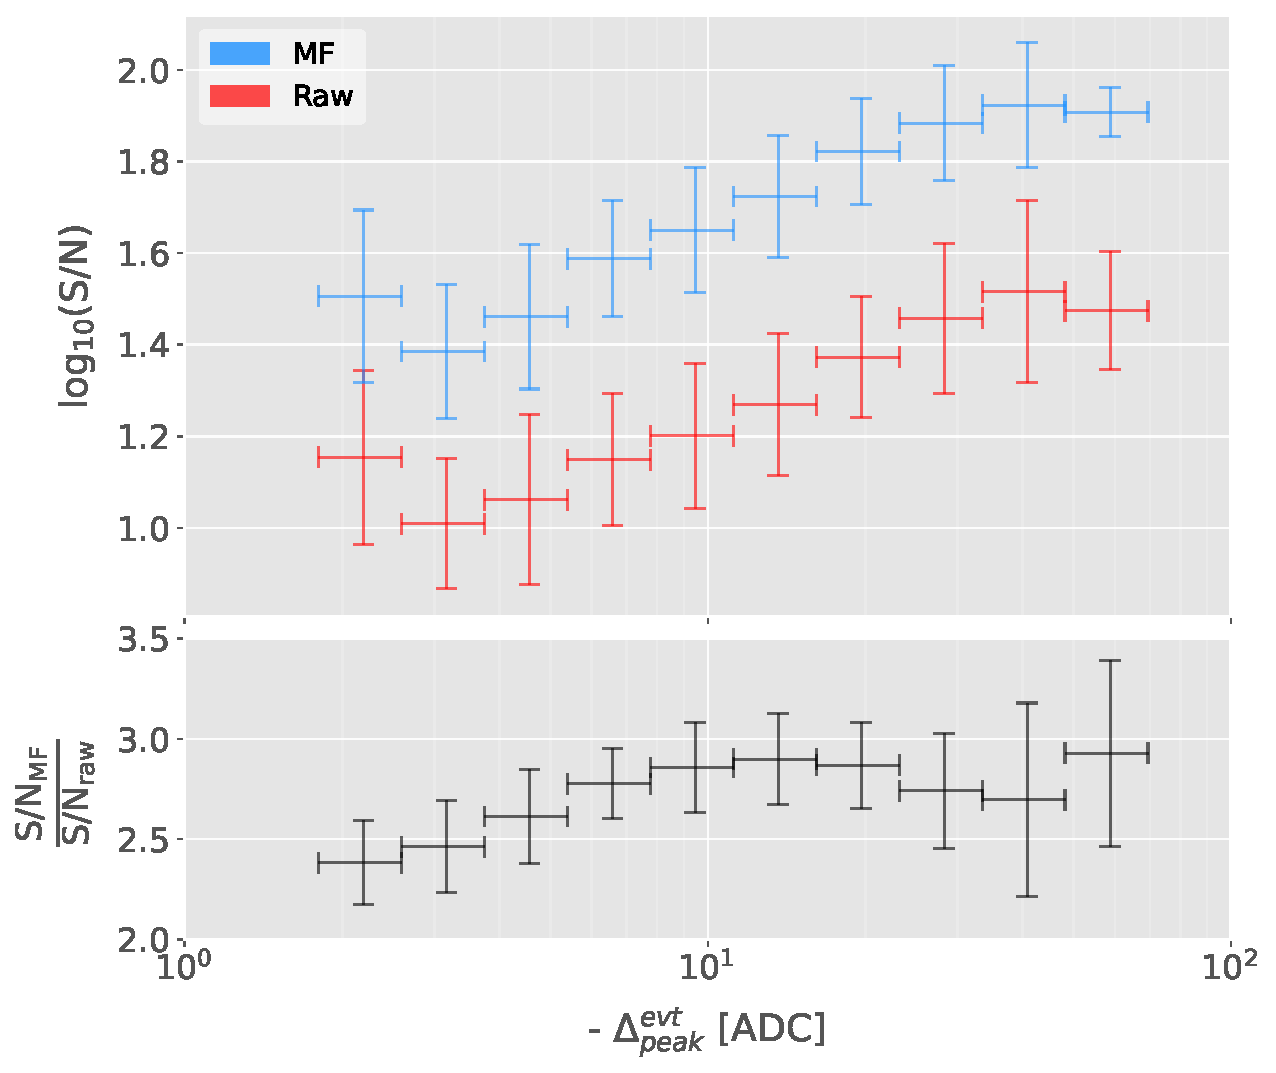
\includegraphics[width=.99\linewidth]{Images/Matched_Filter/deltaPeak_SN_ratio}
	\end{subfigure}
	\caption[Distribution of the peak asymmetry for the monoenergetic muon sample and dependence of the S/N change on the mean peak asymmetry of the event.]{Left panel: peak asymmetry distribution for the case of the monoenergetic $E_{k} = 100 \ \mathrm{MeV}$ muon sample. Each value corresponds to a single bipolar signal peak from a channel in any event. The blue distribution represents the peaks on U plane channels, whereas the red corresponds to signal peaks in V wires. Right panel: relation between the mean peak asymmetry per event with the S/N for U channel waveforms from the $E_{k} = 100 \ \mathrm{MeV}$ muon sample. The top subplot shows the decimal logarithm of the mean S/N for the raw (red) and the matched filtered (blue) waveforms. The bottom subplot contains the mean S/N improvement ratio after the matched filter was applied.}
	\label{fig:asymmetry}
\end{figure}

\begin{table}[h!]
	\centering
	\caption[Characteristic parameters of the two monoenergetic muon events selected for the peak asymmetry study.]{Characteristic parameters of the two monoenergetic muon events selected, relative to the U plane: projected angles in the $xz'$ and $y'z'$ planes, S/N values for the raw and filtered waveforms, mean improvement of the S/N and peak asymmetry.}
	\begin{tabular}{l|llllll}
		& $\theta_{xz'} \ (^{\circ})$ & $\theta_{y'z'} \ (^{\circ})$ & $\mathrm{S/N}_{\mathrm{raw}}$ & $\mathrm{S/N}_{\mathrm{MF}}$ & $\frac{\mathrm{S/N}_{\mathrm{MF}}}{\mathrm{S/N}_{\mathrm{raw}}}$ & $\Delta_{peak} \ (\mathrm{ADC})$ \\[2mm] \hline
		\rule{0pt}{1.1\normalbaselineskip}High (``parallel'') & -1.58                     & -77.76                     & 41.65       & 112.44      & 2.83                          & -35.73                                                          \\[2mm]
		Low (``normal'')  & 76.92                     & -2.56                      & 8.07        & 25.46       & 3.12                          & -10.38                                                         
	\end{tabular}
	\label{tab:case}
\end{table}

One can try to understand better the nature of these two events by looking at the raw and filtered data from some of their active channels. Figure \ref{fig:example_orientation} shows a selection of consecutive raw and filtered U plane waveforms from the event with high S/N (left panel) and the one with low S/N (right panel). To show both collections of waveforms at a similar scale I had to apply a factor of $0.15$ to the waveforms with high S/N. Additionally, next to each waveform I include the values of the raw and matched filtered S/N for the corresponding channel. The first thing to notice is that the amplitude of the signal peaks from the normal track have a much smaller amplitude, and also appear quite distorted when compared to the others. On the other hand, although the matched filtered S/N for each channel are still smaller, the relative improvements are larger than in the parallel case.

A way to quantify the difference between the shape of the waveforms of these two events is using their peak asymmetry. I define the peak asymmetry as the (signed) difference between the positive and the negative peaks of the bipolar shape, i.e.:
\begin{equation}
\Delta_{peak} \equiv h_{+} - h_{-},
\end{equation}
where both heights $h_{+}$ and $h_{-}$ are positive. Figure \ref{fig:asymmetry} (left panel) shows the distribution of this peak asymmetry for all the waveforms corresponding to channels in the U (blue) and V (red) planes for the monoenergetic muon sample. One can see that these distributions are clearly shifted to negative values, with means $\mu_{\Delta}^{\mathrm{U}} = -10.57 \ \mathrm{ADC}$ and $\mu_{\Delta}^{\mathrm{V}} = -5.72 \ \mathrm{ADC}$, respectively. Notice how the peak asymmetry value of the selected event with the high S/N sits at the left tail of the distribution, whereas the corresponding value of the sample with the low S/N lies around the mean.

It is possible to correlate the peak asymmetry with the S/N and the S/N change per event. Figure \ref{fig:asymmetry} (right panel) shows the result of comparing the mean peak asymmetry per event to the averaged raw (red) and matched filtered (blue) S/N per event (top subplot). The horizontal lines sit at the mean value obtained in the fit and represent the width of the $-\Delta_{peak}$ bins used, while the vertical lines indicate one standard deviation around that mean value. Notice how there is an approximate linear relation between the peak asymmetry and the S/N, except for peak asymmetry values bigger than $- 5 \ \mathrm{ADC}$ where the S/N remains constant.

Also, in the bottom subplot of Fig. \ref{fig:asymmetry} (right panel) I show the relation between the peak asymmetry and the mean S/N change. In this case, one can see that there is a clear maximum at $\Delta_{peak} \sim -10 \ \mathrm{ADC}$. As mentioned previously, this is also the value of the mean of the peak asymmetry distribution. In fact, it is expected that our filter favours the signal peaks with the most common values of the peak asymmetry, as this was one of the features I target in our filter coefficient optimisation through the parameter $\delta$.

These results suggest that events with poorer values of the mean S/N, usually associated to non-favourable track orientations, tend to have smaller values of the mean peak asymmetry (in absolute value). Nonetheless, because our matched filters have been optimised to account for these asymmetries, the improvement on the S/N for these events is sizeable if not better than the one for events which already had a high S/N.